\documentclass[xcolor=dvipsnames]{beamer}
\usepackage[T1]{fontenc}
\usepackage[utf8]{inputenc}
\usepackage[english,slovak]{babel}

\usepackage{amsmath}
\usepackage{amsthm}
\usetheme{Pittsburgh}
\useoutertheme{shadow}

\usepackage{graphicx}
\usepackage{caption}
\usepackage{subcaption}

\usepackage{tabularx}

\usepackage{movie15}


\usepackage{listings}
\lstloadlanguages{Ruby}
\lstset{%
basicstyle=\ttfamily\color{black},
commentstyle = \ttfamily\color{red},
keywordstyle=\ttfamily\color{blue},
stringstyle=\color{orange}}



%-------------------------------------------------------------------------------------
\title{\bf Q-learning - umelá inteligencia na obzore?}
\author{Ing. Michal CHOVANEC \\Fakulta riadenia a informatiky}

\date[EURP]{\it Apríl 2016}
\begin{document}

\begin{frame}
\titlepage
\end{frame}


%“a way of programming agents by reward and
%punishment without needing to specify how the
%task is to be achieved”
%[Kaelbling, Littman, & Moore, 96]


%-------------------------------------------------------------------------------------
\begin{frame}{\bf Obsah}

\begin{minipage}{.5\textwidth}

\begin{itemize}
  \item Reinforcement learing
  \item Q-learning algoritmus
  \item Možnosti aproximácie
\end{itemize}

  \end{minipage}%
\begin{minipage}{.5\textwidth}

  \begin{figure}[!htb]
  \centering
  \includegraphics[scale=.8]{../pictures/go.jpg}
  \end{figure}

\end{minipage}

\end{frame}


%-------------------------------------------------------------------------------------
\begin{frame}{\bf Reinforcement learing}

\begin{minipage}{.5\textwidth}

\begin{itemize}
  \item Zistenie stavu
  \item Výber akcie
  \item Vykonanie akcie
  \item Prechod do ďalšieho stavu
  \item Získanie odmeny alebo trestu
  \item Učenie sa zo získanej skúsenosti
\end{itemize}

  \end{minipage}%
\begin{minipage}{.5\textwidth}

  \begin{figure}[!htb]
  \centering
  \includegraphics[scale=.8]{../diagrams/agent.png}
  \end{figure}

\end{minipage}

\end{frame}

\begin{frame}{\bf Výhody}

Definuje sa čo robiť, nie ako to robiť
\begin{itemize}
\item vďaka odmeňovacej funkcií
\item agent sa môže naučiť všetky detaily problému
\end{itemize}

Lepšie konečné riešenie
\begin{itemize}
\item založené na skutočnej skúsenosti, nie skúsenosti programátora
\item treba menej ľudského času na nájdenie dobrého riešenia
\end{itemize}


\end{frame}


%-------------------------------------------------------------------------------------
\begin{frame}{\bf Markovov rozhodovací proces}

  \begin{figure}[!htb]
  \centering
  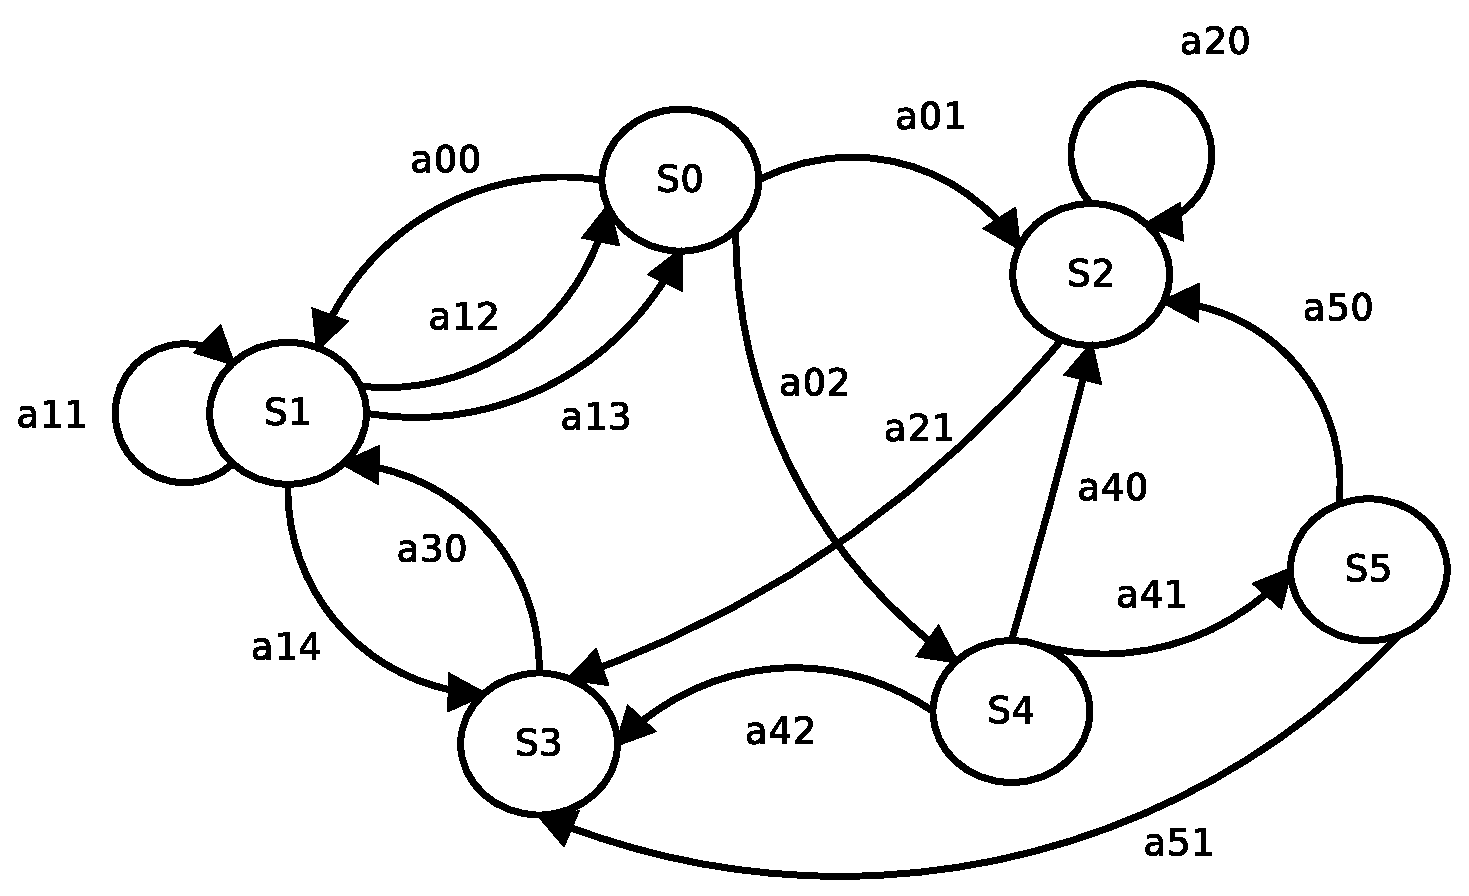
\includegraphics[scale=.4]{../diagrams/markovov_process.eps}
  \end{figure}

\end{frame}




%-------------------------------------------------------------------------------------
\begin{frame}{\bf Experiment s jedným stavom - nanoQ learning}
  Plánovanie pohybu robota - aký krok má robot vybrať?
  Dostupné akcie : vľavo, vpravo, vpred, (vzad)

  \begin{minipage}{.5\textwidth}

    \begin{figure}[!htb]
    \centering
    \includegraphics[scale=.3]{../pictures/kilobot.jpg}
    \end{figure}


    \end{minipage}%
  \begin{minipage}{.5\textwidth}

    \begin{figure}[!htb]
    \centering
    \includegraphics[scale=.1]{../pictures/apds9930.jpg}
    \end{figure}

  \end{minipage}

  Robot s jednoduchým senzorom
  \begin{itemize}
  \item smer nie je známy
  \item známa je len vzdialenosť
  \item šum
  \end{itemize}

\end{frame}





%-------------------------------------------------------------------------------------
\begin{frame}{\bf Experiment s jedným stavom - nanoQ learning}


  \begin{minipage}{.5\textwidth}

    \begin{itemize}
      \item Najjednoduhší prípad Q-learning algoritmu
      \item Reward zadaný dvoma hodnotami :
              \begin{itemize}
                \item situácia sa zlepšuje $+1$
                \item situácia sa zhoršuje $-1$
              \end{itemize}
      \item Voliteľná prevdepodobnosť $p \in \langle 0, 4 \rangle$ náhodnej zmeny rewardu - šum
    \end{itemize}


  \end{minipage}%
  \begin{minipage}{.5\textwidth}

    \begin{figure}[!htb]
    \centering
    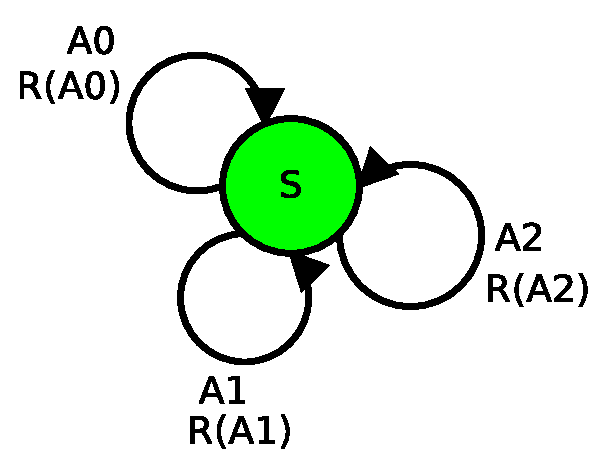
\includegraphics[scale=.5]{../diagrams/single_state.eps}
    \end{figure}

  \end{minipage}

  \begin{equation}
  Q_n(A(n)) = R(n) + \gamma  \max_{a'(n-1) \in \mathbb{A}} Q_{n-1}(a'(n-1))
  \label{eq:nano_q_func}
  \end{equation}


\end{frame}



%-------------------------------------------------------------------------------------
\begin{frame}{\bf Výber akcie}

\begin{equation}
a(n) =
\left\{
	\begin{array}{ll}
		a(n-1)  & ak \ Q_{n-1}(a(n-1)) > 0 \\
    random() & inak
	\end{array}
\right.
\label{eq:q_nano_action_selection}
\end{equation}

  \begin{figure}[!htb]
  \centering
  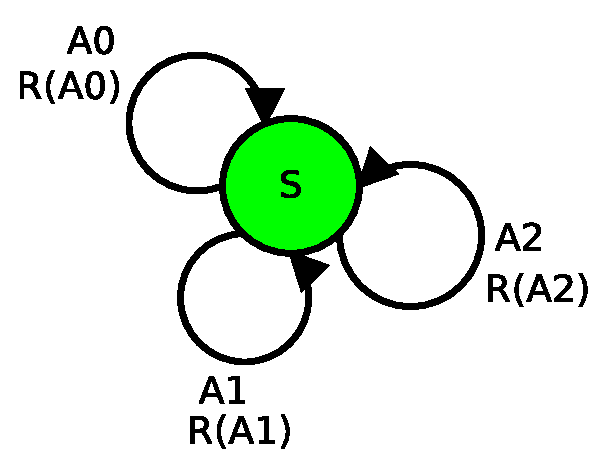
\includegraphics[scale=.5]{../diagrams/single_state.eps}
  \end{figure}
\end{frame}

%-------------------------------------------------------------------------------------
\begin{frame}{\bf Výsledky}


  \begin{minipage}{.5\textwidth}

    \begin{figure}[!htb]
    \centering
    \includegraphics[scale=.2]{../../results_q_learning/nano_q_learning/result_00/robot_path.png}
    \caption{Dráha robotov pre $\gamma = 0.7 p = 0.0$}
    \label{img:nano_q_result_00_path}
    \end{figure}


  \end{minipage}%
  \begin{minipage}{.5\textwidth}

    \begin{figure}[!htb]
    \centering
    \includegraphics[scale=.2]{../../results_q_learning/nano_q_learning/result_04_02/robot_path.png}
    \caption{Dráha robotov pre $\gamma = 0.7 p = 0.4$}
    \label{img:nano_q_result_04_2_path}
    \end{figure}

  \end{minipage}

\end{frame}



%-------------------------------------------------------------------------------------
\begin{frame}{\bf Výsledky}


  \begin{minipage}{.5\textwidth}

    \begin{figure}[!htb]
    \centering
    \includegraphics[scale=.2]{../../results_q_learning/nano_q_learning/result_04_03/robot_path.png}
    \caption{Dráha robotov pre $\gamma = 0.9 p = 0.4$}
    \label{img:nano_q_result_04_3_path}
    \end{figure}


  \end{minipage}%
  \begin{minipage}{.5\textwidth}

    \begin{figure}[!htb]
    \centering
    \includegraphics[scale=.2]{../../results_q_learning/nano_q_learning/result_04_04/robot_path.png}
    \caption{Dráha robotov pre $\gamma = 0.98 p = 0.4$}
    \label{img:nano_q_result_04_4_path}
    \end{figure}

  \end{minipage}

\end{frame}


%-------------------------------------------------------------------------------------
\begin{frame}{\bf Výsledky - zhrnutie}
Komplexné vyšetrenie závislosti $\gamma$ a $p$. Znázornenie funkcie vzdialenosti od pohyblivého cieľa po 25000 krokoch robota, priemer z 32 robotov

\begin{figure}[!htb]
\centering
\includegraphics[scale=.35]{../../results_q_learning/nano_q_learning/summary_result_average_error_map.png}
\caption{Priemerná chyba 32 robotov po 25000 iteráciach}
\label{img:nano_q_summary}
\end{figure}

\end{frame}








%-------------------------------------------------------------------------------------
\begin{frame}{\bf Q-learning algoritmus}

Daná je funkcia ohodnotení

\begin{equation}
Q(s(n),a(n)) = R(s(n),a(n)) + \gamma \max_{a(n-1) \in \mathbb{A}} Q(s(n-1), a(n-1)) \nonumber
\end{equation}

kde \\

\begin{itemize}
 \item $R(s(n),a(n))$ je odmeňovacia funkcia s hodnotami v $\langle -1, 1 \rangle$, \\
 \item $Q(s(n-1),a(n-1))$ je odmeňovacia funkcia v stave $s(n-1)$ pre akciu $a(n-1)$, \\
 \item $\gamma$ je odmeňovacia konštanta a platí $\gamma \in (0, 1)$.
\end{itemize}

\end{frame}


%-------------------------------------------------------------------------------------
\begin{frame}{\bf Odmeňovacia funkcia}

\begin{figure}[!htb]
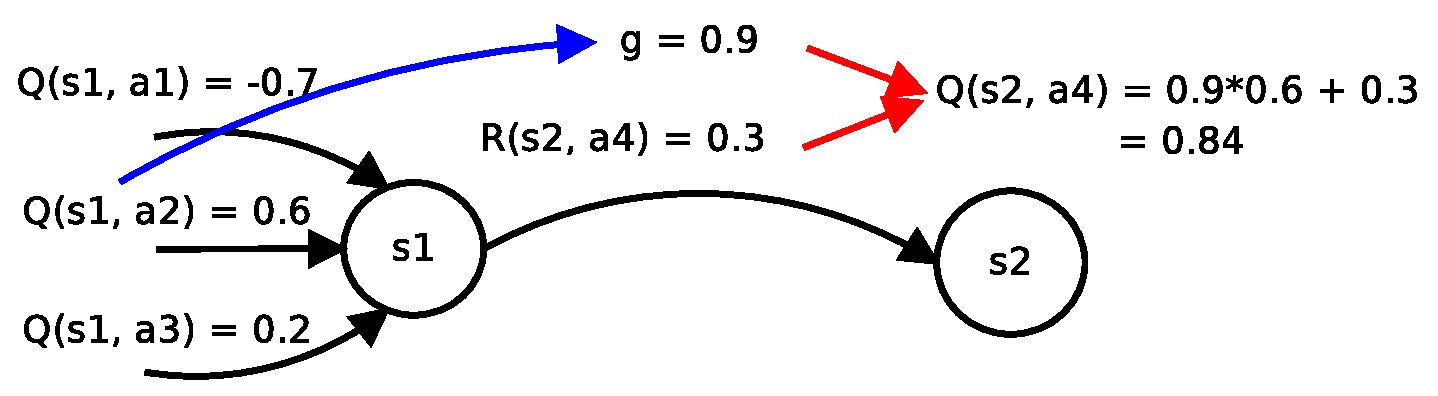
\includegraphics[scale=.4]{../diagrams/q_learning_detail.eps}
\end{figure}

\end{frame}

%-------------------------------------------------------------------------------------
\begin{frame}{\bf Rozsiahly stavový priestor - ukážka požadovaného tvaru funkcie}

\begin{figure}[!htb]
\centering
\includegraphics[scale=.39]{../../results_q_learning/map_1/function_type_0/iterations_10/q_learning_result.png}
\caption{reference table}
\end{figure}

\end{frame}




%-------------------------------------------------------------------------------------
\begin{frame}{\bf Implementačné problémy}

Problémy tabuľkovej interpretácie $Q(s(n), a(n))$ :

\begin{itemize}
\item pre veľké ${n_s}$  alebo  ${n_a}$ narastajú pamäťové nároky,
\item o nevyplnených $Q(s(n), a(n))$ nevieme povedať nič,
\item pre rozsiahle stavové priestory ťažko vypočítateľné,
\item ako aproximovať $Q(s(n), a(n))$?
\end{itemize}

Je možné zostaviť neurónovú sieť, ktorá sa dá naučiť lokálne?

\end{frame}


\begin{frame}{\bf Experiment s novou bázickou funkciou}

Experimentálne sa zitili typické rysy funkcie pre

\begin{equation*}
Q_{n}(s(n),a(n)) = R(s(n),a(n)) + \gamma \max_{a(n-1) \in \mathbb{A}} Q_{n-1}(s(n-1), a(n-1))
\label{eq:q_learning}
\end{equation*}

\begin{figure}[]
\center
\includegraphics[scale=.35]{../pictures/peak_hill_function.png}
\caption{Znázornenie predmetnej funkcie}
\label{img:peak_hill_funcion}
\end{figure}

\end{frame}

\begin{frame}{\bf Experiment s novou bázickou funkciou}

{\bf P}eak and {\bf H}ill funkcia

\begin{align}
P_i(s(n), a(n)) &=
\left\{
	\begin{array}{ll}
		r_{ai}  & if \ s(n) = \alpha^1_i \\
		0 & inak
	\end{array}
\right. \\
  H_j(s(n), a(n)) &= w_{aj} e^{ -\beta_{aj} \sum\limits_{i=1}^{n_s}{(s_i(n) - \alpha^2_{aji})^2 }} \\
  Q(s(n), a(n)) &= \sum\limits_{i=1}^{I} P_i(s(n),a(n)) + \sum\limits_{j=1}^{J} H_j(s(n), a(n))
  \label{eq:peak_hill}
\end{align}

kde \\
$\alpha^1_j$ sú oblasti kde $H_j(s(n))$ nadobúda nenulové hodnoty \\
$\alpha^2_j$ sú oblasti pre ktoré $f_j(\boldmath{s(n), a(n)})$ nadobúda maximum \\
$r_{ai}$ je hodnota okamžitej odmeny $R(s(n))$ v tomto stave \\
$w_{aj}$ je váha a zobovedá veľkosti maxima resp. minima pre fukciu \\
$\beta_{aj}$ je strmosť, a platí $\beta > 0$ \\
$I$ a $J$ sú počty bázických funkcií \\

\end{frame}


%-------------------------------------------------------------------------------------
\begin{frame}{\bf Schéma priebehu experimentov}

\begin{figure}[!htb]
\centering
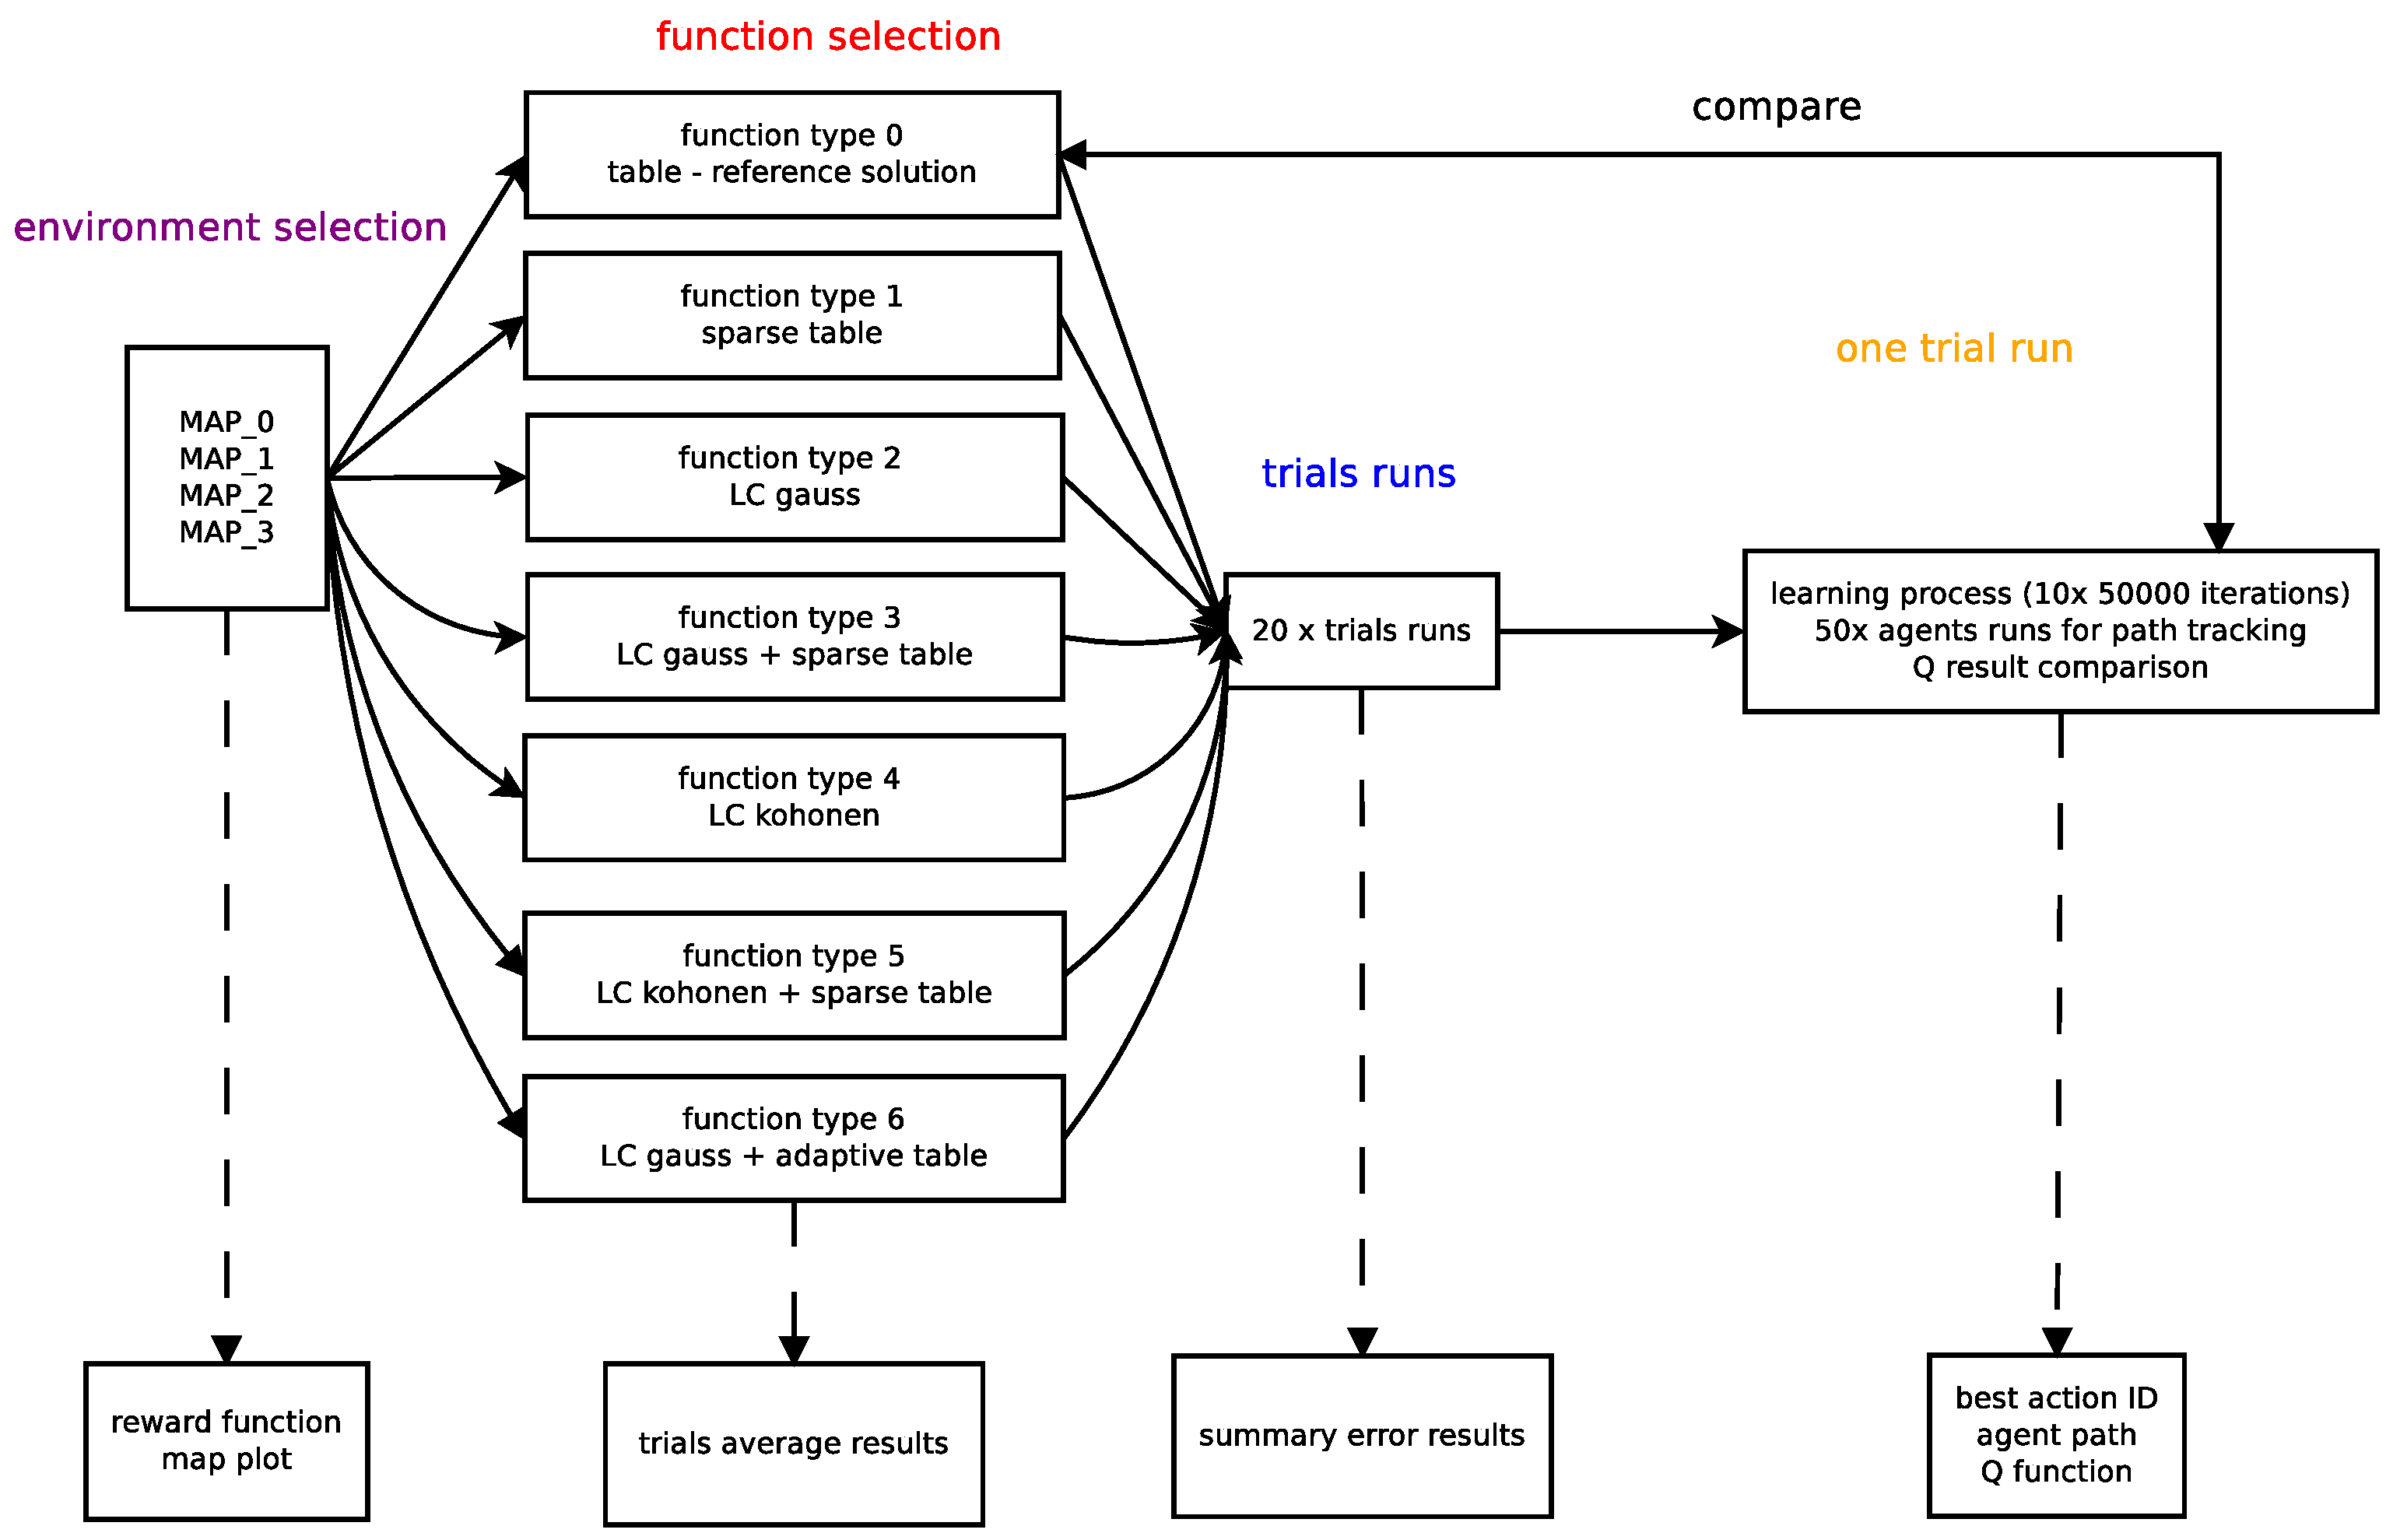
\includegraphics[scale=.22]{../diagrams/experiment_map_q_learning.eps}
\end{figure}

\end{frame}



\begin{frame}{\bf Porovnanie s ostatnými}

\begin{figure}[!htb]
\centering
\includegraphics[scale=.4]{../../results_q_learning/map_2/trials_average_results.png}
\end{figure}

\end{frame}


\begin{frame}{\bf Porovnanie s ostatnými}

\begin{minipage}{.5\textwidth}

  \begin{figure}[!htb]
  \centering
  \includegraphics[scale=.2]{../../results_q_learning/map_2/function_type_2/iterations_10/agents_path_surface.png}
  \caption{Dráha robotov, funkcia 2 - Gauss}
  \label{img:knn_path}
  \end{figure}


\end{minipage}%
\begin{minipage}{.5\textwidth}

  \begin{figure}[!htb]
  \centering
  \includegraphics[scale=.2]{../../results_q_learning/map_2/function_type_6/iterations_10/agents_path_surface.png}
  \caption{Dráha robotov, funkcia 6 - Peak and Hill}
  \label{img:peak_and_hill_path}
  \end{figure}

\end{minipage}

\end{frame}

\begin{frame}{\bf Doplnkový experiment}

\begin{figure}[!htb]
\centering
\includegraphics[scale=.05]{../pictures/motoko_aftermath_front.jpg}
\label{img:motoko_robot_photo}
\end{figure}

\end{frame}


\begin{frame}{\bf Doplnkový experiment}

Bloková schéma robota

\begin{figure}[!htb]
\centering
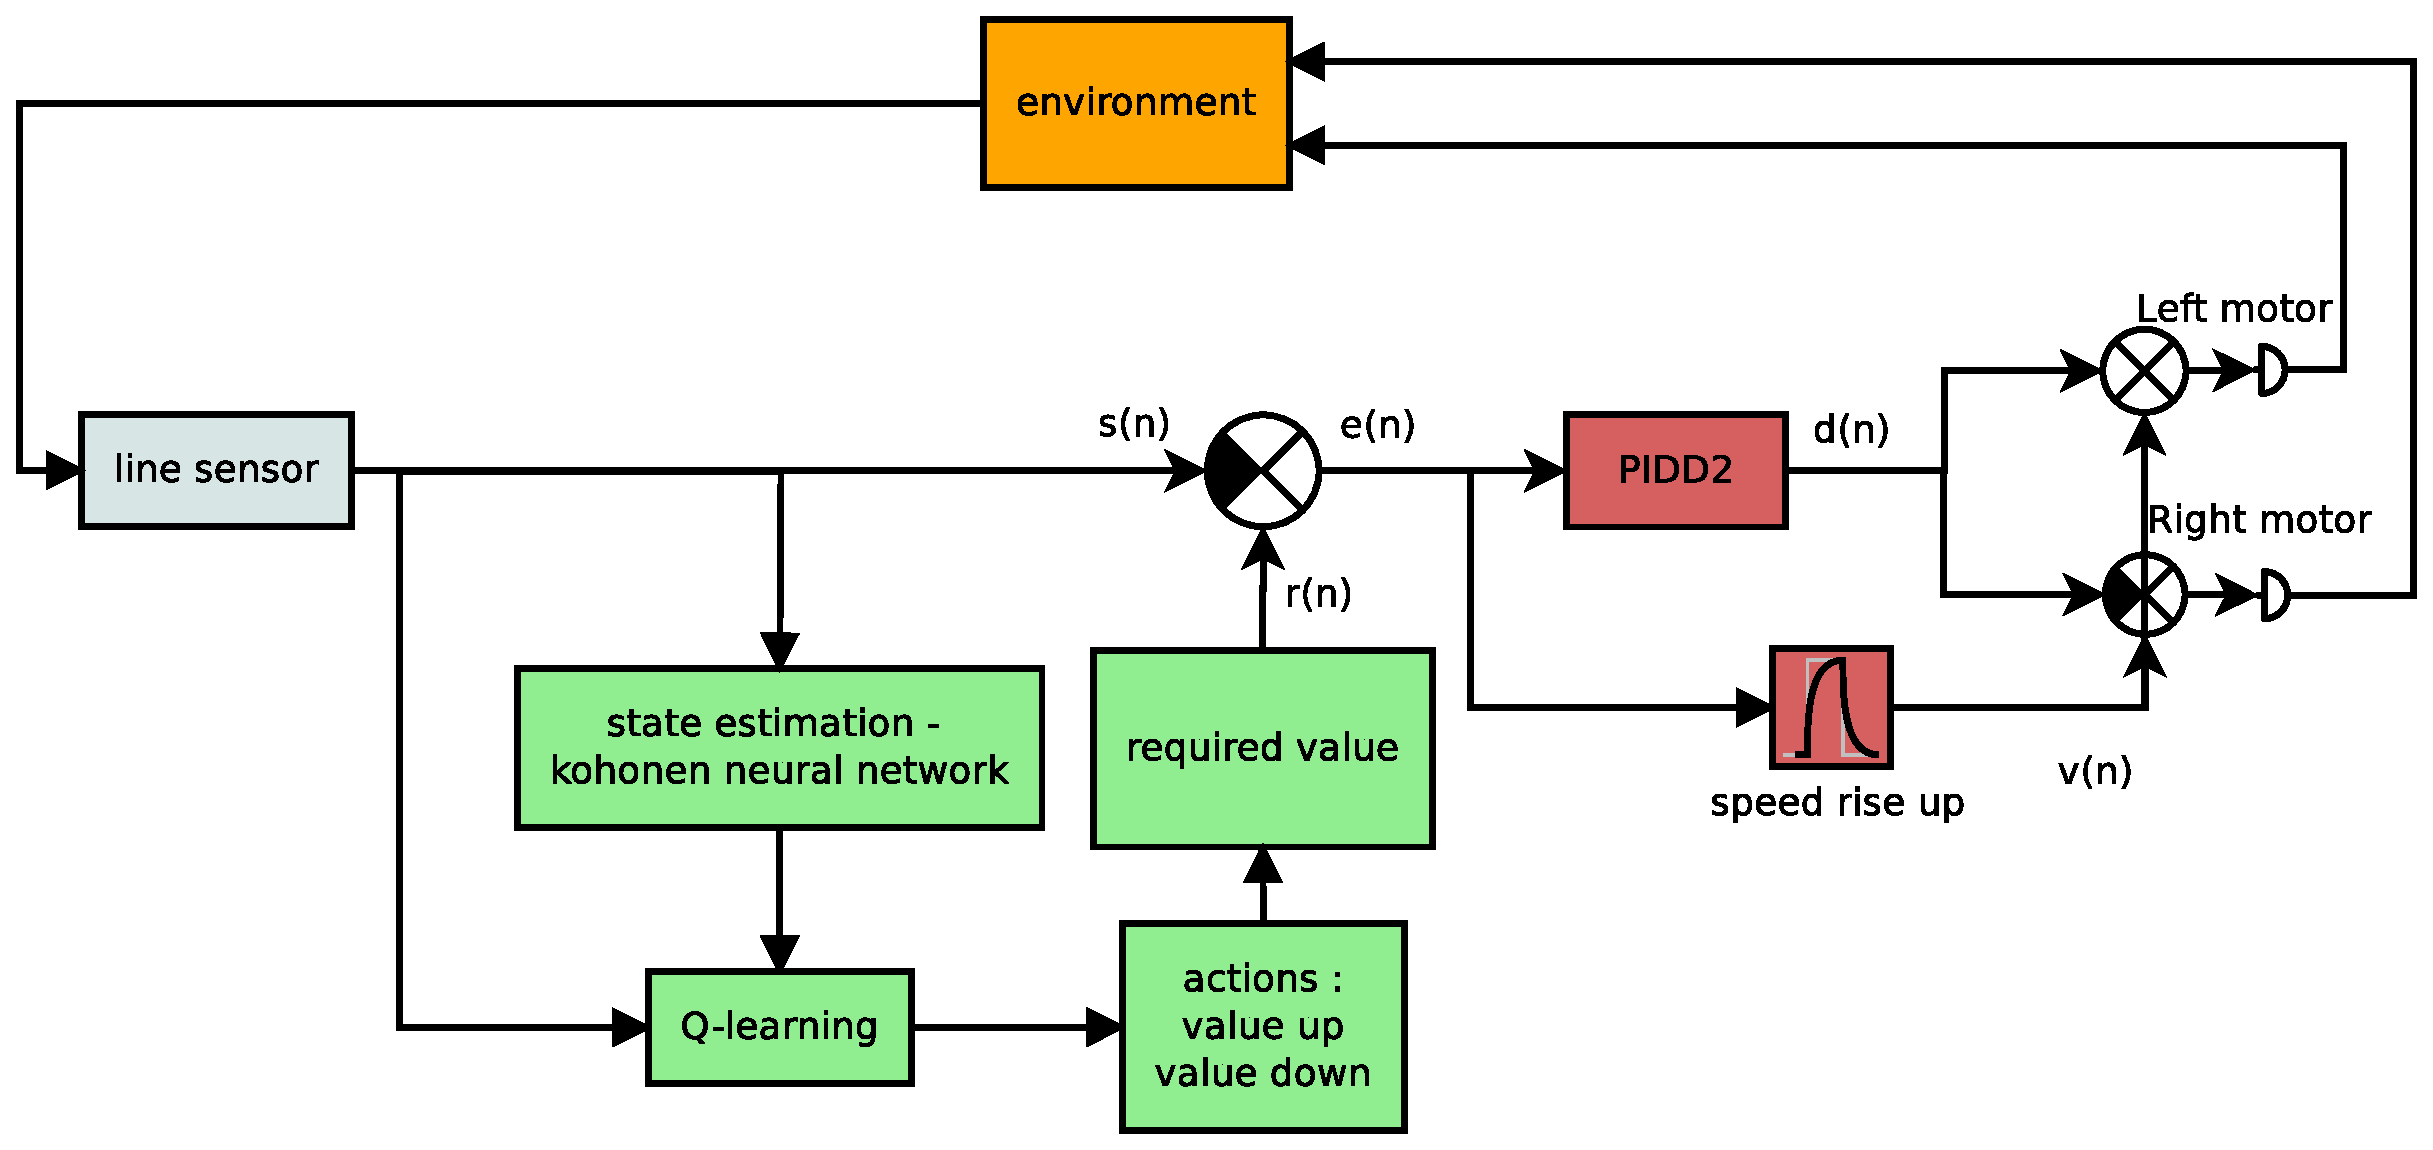
\includegraphics[scale=.25]{../diagrams/motoko_robot_block.eps}
\label{img:motoko_robot_block}
\end{figure}

\end{frame}




%-------------------------------------------------------------------------------------
\begin{frame}{\bf Ďakujem za pozornosť}

\centerline{michal.chovanec@yandex.ru}
\centerline{https://github.com/michalnand/q\_learning}

\begin{figure}[!htb]
\centering
\includegraphics[scale=.2]{../pictures/me_ferrata.jpg}
\end{figure}

\end{frame}














\end{document}
